




\begin{marginfigure}
\centering
\frame{\includegraphics[width=\linewidth]{"images/2013/other-finds-2013/oli-fire".jpg}}
\label{Olifire}
\caption{On the last night on top of the mountain, all perishable food is ritually burned as Oliver Myerscough demonstrates with flour--- Kate Smith}
\end{marginfigure}

\section{Below Balamory}

\margininbox{Balamory}{\begin{itemize}
    \item Clare Tan
    \item Grega Maffi
    \item Iztok Mozir
    \end{itemize}}
    
\subsection{06/08/2013}
Exciting night of pushing yesterday. \passage{Clapton} pitch is a massive space. Effectively like two shafts right next to each other. We drop the shorter one. Couple of leads at the bottom. One has a bedding plane squeeze that stopped Maffi, it follows water to a small pitch, might join up with something off the other half of \passage{Clapton}.
We mainly pushed the other lead, schematic on facing page. It's still open and going.Unfortunatley when we started to survey we discovered a crack in the clino glass. Which is why the tentative passage name is now \passage{Crack Shack} [ed. not on page reads `Renamed \passage{Pick Your Poison}]. There's also alot of black sandy silt deposition in our passage, plus its in keeping with the cocaine theme...
Going back today to survey waiting for day trainers to arrive, listening to music, writing this t put off pissing....I really like caving and camping underground...
P.S. none of the leads were killed during this push!!!!
\name{Clare Tan}

\begin{pagefigure}
      \checkoddpage \ifoddpage \forcerectofloat \else \forceversofloat \fi
      \centering
    \begin{subfigure}[t]{\textwidth}
    \centering
        \frame{\includegraphics[width=\linewidth]{"images/2013/other-finds-2013/lethe_sifon_2".jpg}} 
        \caption{} \label{lethe sifon 2}
    \end{subfigure}
    
          \vspace{0.3cm}
          
    \begin{subfigure}[t]{0.555\textwidth}
        \centering
        \frame{\includegraphics[width=\linewidth]{"images/2013/other-finds-2013/clare_in_lethe".jpg}} 
        \caption{} \label{clare in lethe}
    \end{subfigure}
    \hfill
    \begin{subfigure}[t]{0.418\textwidth}
        \centering
        \frame{\includegraphics[width=\linewidth]{"images/2013/other-finds-2013/lethe_canyon".jpg}} 
        \caption{} \label{lethe canyon}
    \end{subfigure}

    \caption{
    \emph{(a)} The cascading steam from \protect\passage{Brezno Slapov} ends at an ominous sump (-802m)
    \emph{(b)} Clare Tan navigates through the stream and canyon passage below \protect\passage{Brezno Slapov}.
    \emph{(c)} Water from the stream passage accumulates in deep pools --- Iztok Mozir }
\end{pagefigure}

\begin{pagefigure}
      \checkoddpage \ifoddpage \forcerectofloat \else \forceversofloat \fi
      \centering
              \frame{\includegraphics[width=\linewidth]{"images/2013/other-finds-2013/kate-end-of-expo-2013".jpg}} 
       \label{end expo}
  \caption{Marjan Koblu\v{c}ar, Slavica Klobu\v{c}ar, Clare Tan, Nadine Kalmoni, Sam Page, Janet Cotter, Chris Keeley, Kate Smith, David Kirkpatrick, Rhys Tyers, Fiona Hartley, Dave Wilson, Oliver Myerscough --- Tim Child }
\end{pagefigure}


\subsection{07/08/2013}
Went back to \passage{Clapton} yesterday to survey what we found the previous trip ~200m added to this years total. There are so many leads there we called it \passage{Pick Your Poison}. Will be dreaming about it now for the next 11 months...
I guess this is now my last few hours in camp. It's been a great expo of caving for me - many thanks to all my pushing/camping partners: Saber, Izi, Rhys and Maffi for the excellent trips and company. Thanks also to all who have camped at \passage{X-Ray} for the laughs and great conversation.
Almost can;t believe another expo is drawing to a close...caving-wise I feel thoroughly satiated, but I've enjoyed myself so much that I don't want it to end. Ah well, there's always next year, and the year after, and the year after....I wonder if I'll still be here in 10 years?
I should really go to sleep but my body doesn't want to cooperate....Maybe it's time to read Tetley's 15 page epic (from earlier in the expo.) \name{Clare Tan}
\vspace{70pt}

Still no inspiration, I guess Clare Tan has drained out of me even this, nor only all energy, while trying to figure out how to squeeze through thos passages we've found. Anyway it is the last day in \passage{X-Ray} this year. Wish this refuge was open the whole year. Aja! I want to thank Dave Wilson for the hint on \passage{Balamory}. He made possible the biggest discovery this year! And with this he also gave Erik and me the sensation of pioneers. Thanks Dave! (well this sensation we get every time we push something nice but this one could be compared with findings of Columbus, Marco Polo, Juri Gagarin :) ) Thank you Erik, thank you Clare Tan. Thank you everyone that made Mig adventures possible. Over an out.
\name{Grega Maffi}

\section{At the end of Atlantis} 
Pushed \passage{Brezno Slapov} with Izi last night, it was a great trip. 

Dropped a couple of pitches to get to a canyon/rift with a stream, followed it and eventually got to a sump. But taking a left turn down and inlet leads to the base of another wet pitch and a continuation of passage, but is was wet and we didn't go on. \name{Clare Tan}



\begin{figure*}
\begin{tikzpicture}
\node [table] (box){%
    \begin{minipage}{\linewidth}
    \centering
    \begin{tabular}{lrrrr}
    Sector & \multicolumn{1}{l}{Passage name} & Survey length (m) & Stations & Average leg (m) \\ \midrule
    \multirow{2}[0]{*}{Apollo} & \multicolumn{1}{l}{Apollo Traverse} & 21.63 & 5     & 5.41 \\
          & \multicolumn{1}{l}{Beetlejuice} & 55.46 & 9     & 6.93 \\ \midrule
    \multirow{5}[0]{*}{Balamory} & \multicolumn{1}{l}{Bingo Granny} & 21.06 & 5     & 5.27 \\
          & \multicolumn{1}{l}{Clapton} & 51.04 & 11    & 5.10 \\
          & \multicolumn{1}{l}{Kokain Lab} & 69.8  & 12    & 6.35 \\
          & \multicolumn{1}{l}{Kokain Rute} & 113.09 & 21    & 5.65 \\
          & \multicolumn{1}{l}{Pick Your Poison} & 191.66 & 28    & 7.10 \\ \midrule
    Kamikaze & \multicolumn{1}{l}{Rural Underground} & 101.29 & 23    & 4.60 \\ \midrule
    \multirow{4}[0]{*}{Lower Pleasures} & \multicolumn{1}{l}{Curiouser and Curiouser} & 69.42 & 15    & 4.96 \\
          & \multicolumn{1}{l}{Curiouser and Curiouser 2} & 35.45 & 14    & 2.73 \\
          & \multicolumn{1}{l}{Slinging in the Rain} & 86.01 & 17    & 5.38 \\
          & \multicolumn{1}{l}{Labyrinth} & 95.94 & 31    & 3.20 \\ \midrule
    \multirow{6}[0]{*}{Stuck in Paradise} & \multicolumn{1}{l}{Hash} & 39.64 & 14    & 3.05 \\
          & \multicolumn{1}{l}{Hash2} & 26.07 & 8     & 3.72 \\
          & \multicolumn{1}{l}{Hash3} & 21.4  & 9     & 2.68 \\
          & \multicolumn{1}{l}{Lethe} & 138.97 & 30    & 4.79 \\
          & \multicolumn{1}{l}{RCC passage of the year} & 26.5  & 7     & 4.42 \\
          & \multicolumn{1}{l}{We're not Alone} & 39.96 & 7     & 6.66 \\ \midrule
    \multirow{8}[0]{*}{Xanadu } & \multicolumn{1}{l}{500m} & 15.59 & 7     & 2.60 \\
          & \multicolumn{1}{l}{Cuckoo's Nest} & 220.73 & 41    & 5.52 \\
          & \multicolumn{1}{l}{Dwarf Pine} & 33.2  & 6     & 6.64 \\
          & \multicolumn{1}{l}{Hydrophobia} & 63.42 & 11    & 6.34 \\
          & \multicolumn{1}{l}{Rejuvenation Rift} & 103.39 & 29    & 3.69 \\
          & \multicolumn{1}{l}{Straightjacket} & 24.31 & 11    & 2.43 \\
          & \multicolumn{1}{l}{Time Bandits} & 126.56 & 22    & 6.03 \\
          & \multicolumn{1}{l}{Xanadon't} & 34.28 & 12    & 3.12 \\ \midrule
          &       &       &       &  \\
    \textbf{Total} &       & \textbf{1825.87} &       &  \\
    \end{tabular}%
  \label{tab:addlabel}%
  \end{minipage} };
\node[tabletitle, right=10pt] at (box.north west) {Number crunching};
\end{tikzpicture}
\end{figure*}


\begin{pagesurvey}
\centering
\frame{\includegraphics[width=\textheight, angle=270]{"images/2013/other-finds-2013/2013plan".pdf}}
\caption[2013 Plan Survey]{2013 Plan Survey}
\label{plan 2013}
\end{pagesurvey}

\begin{pagesurvey}
\centering
\frame{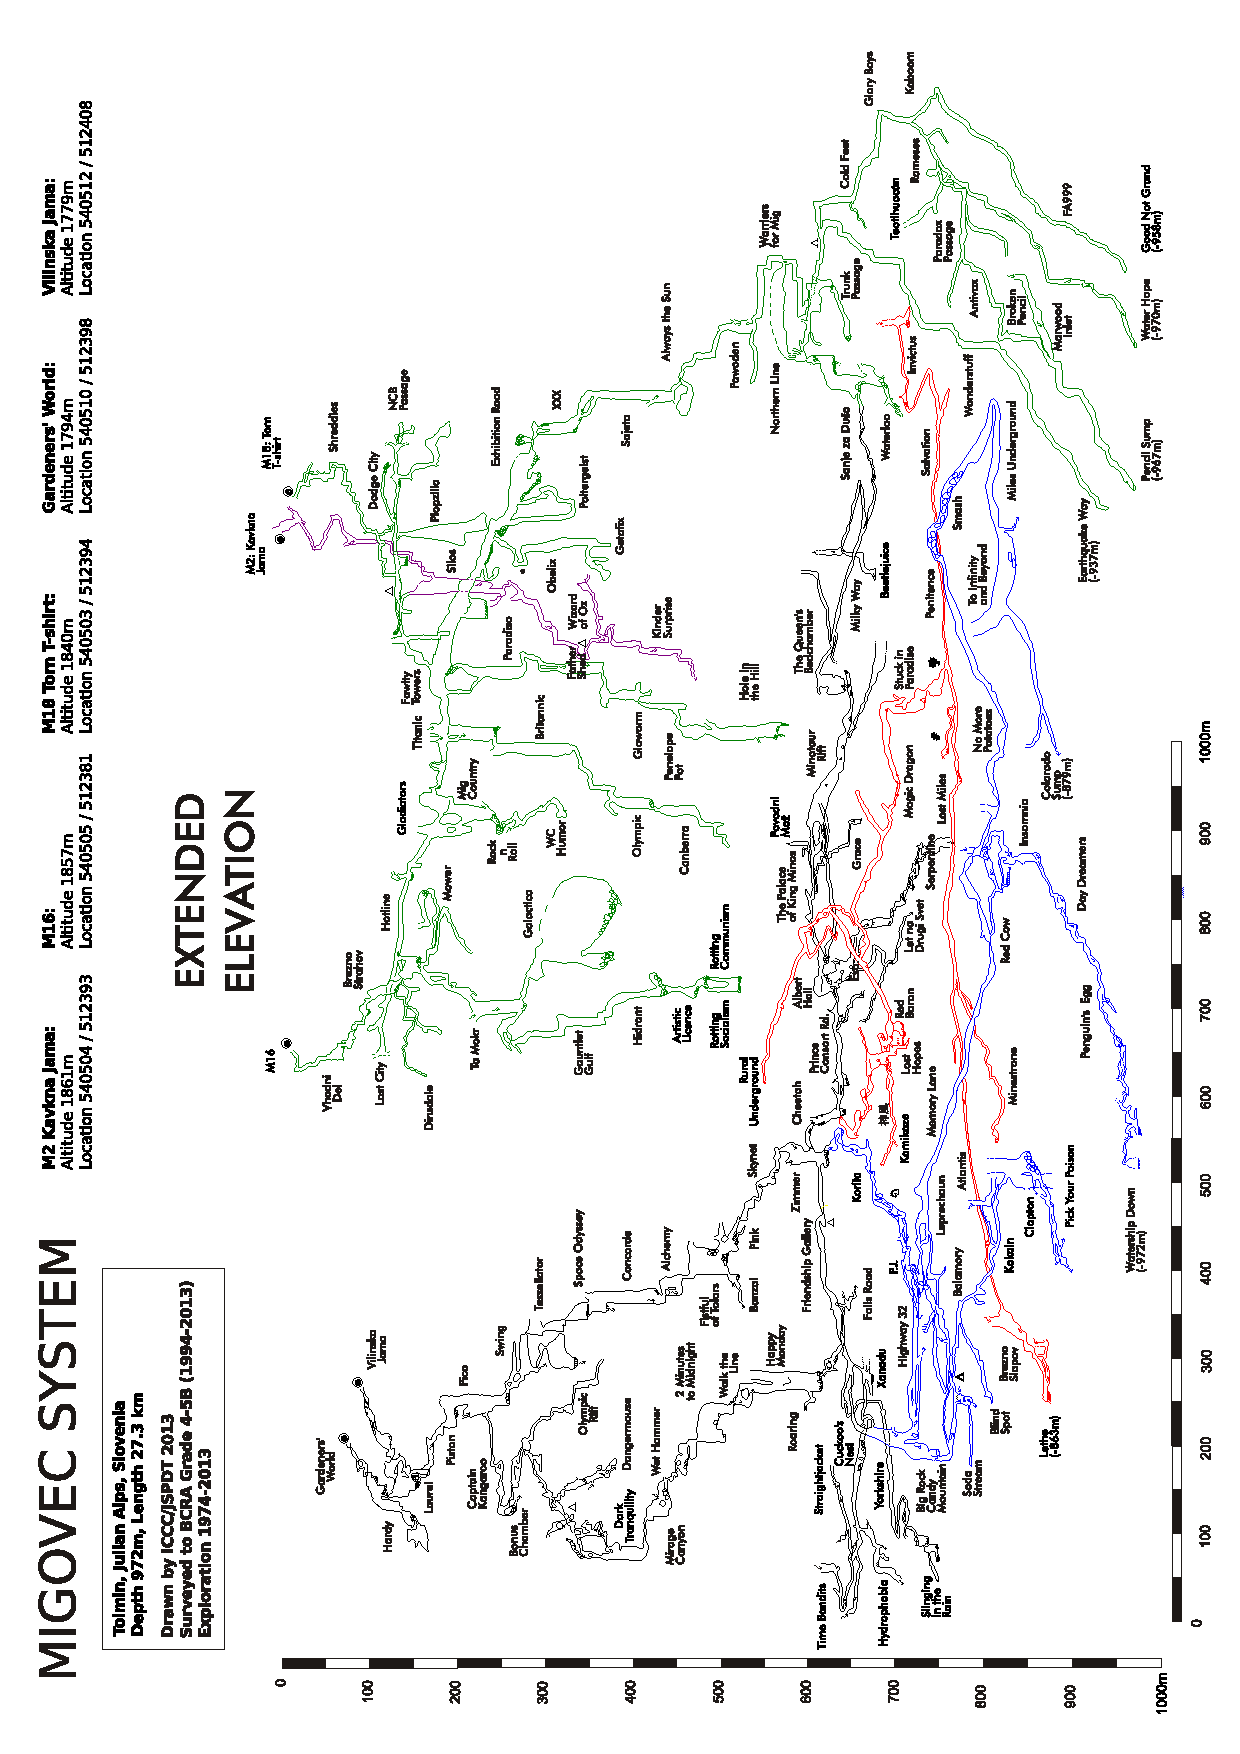
\includegraphics[height=\textheight]{images/2013/other-finds-2013/ee2013.pdf}}
\caption[2013 Extended Elevation]{2013 Extended elevation}
\label{EE 2013}
\end{pagesurvey}
